\documentclass{article}

\input{../../../../../latex_preambule_style/preambule}
\input{../../../../../latex_preambule_style/styleCoursCycle4}
\input{../../../../../latex_preambule_style/styleExercices}
%\input{../../../../../latex_preambule_style/bas_de_page_animation}
\input{../../../../../latex_preambule_style/bas_de_page_cycle4_sans_pagination}
\input{../../../../../latex_preambule_style/algobox}





%%%%%%%%%%%%%%%  Indentation  %%%%%%%%%%%%%%%%%%
\parindent=0pt
%%%%%%%%%%%%%%%%%%%%%%%%%%%%%%%%%%%%%%%%%%%%%%%%

\begin{document}
\begin{titre}[Aide : Geogebra]

\Titre{Espace et Géométrie}{3}
\end{titre}

\sectioncolor{eduscol4B}{Construire un cube}


\subsubsection{Préalable}

\begin{minipage}{0.48\linewidth}
\'A l'aide de l'onglet \touche{Affichage}, cocher :

\begin{description}
\item[Graphique 3D]
\end{description}

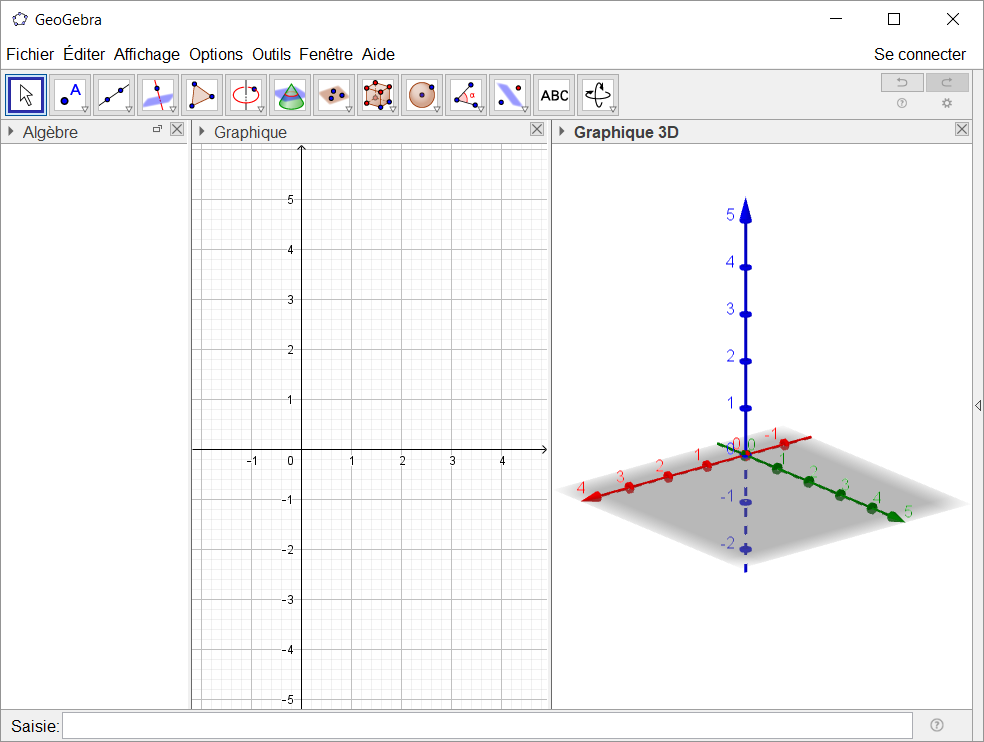
\includegraphics[scale=0.3]{atelier6.png} 

\end{minipage}
\hfill
\begin{minipage}{0.48\linewidth}
Fermer les fenêtres Algèbre et Graphique.


Pour enlever le plan gris et les axes du repère 3D :

\begin{enumerate}
\item Cliquez droit sur la fenêtre \textbf{Graphique 3D} 
\item La fenêtre contextuelle ci-dessous va apparaitre  

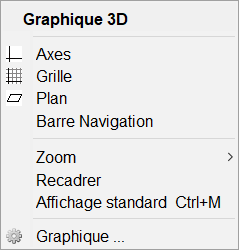
\includegraphics[scale=0.5]{atelier000.png}
\item Décocher : Axes et Plan
\end{enumerate}

\end{minipage}


\paragraph{1. Création du cube}

\begin{minipage}{0.73\linewidth}
\begin{enumerate}
\item Sélectionner la fenêtre \textbf{Graphique 3D} en cliquant sur la fenêtre
\item Placer deux points distincts avec l'icône 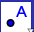
\includegraphics[scale=0.5]{atelier0.png} 
\item Chercher parmi les icones, l'icone Cube et la sélectionner. 
\item Sélectionner les 2 points construits à l'étape 2. Le cube apparait.
\end{enumerate}
\end{minipage}
\hfill
\begin{minipage}{0.25\linewidth}
\begin{Rq}
Pour construire un autre solide, il faut utiliser la commande (icone) appropriée.
\end{Rq}
 \end{minipage}
 
\paragraph{2. Avec des coordonnées}
 
\begin{minipage}{0.73\linewidth}
Pour placer un point dans l'espace, on peut utiliser ces coordonnées. On écrit $A(2;3;4)$. Cela signifie que son abscisse est égale à  2, son ordonnée est égale à  3 et sa cote(ou altitude) est égale à 4.

\begin{enumerate}
\item Sélectionner la fenêtre \textbf{Graphique 3D} en cliquant sur la fenêtre
\item Dans la barre de saisie (en bas de l'écran), écrire :  A=(2,3,4)  . Le point A apparait.
\item Construire alors un autre point avec ses coordonnées. 
\item Chercher parmi les icones, l'icone Cube et la sélectionner. 
\item Sélectionner les 2 points construits à l'étape 2. Le cube apparait.
\end{enumerate}
\end{minipage}
\hfill
\begin{minipage}{0.25\linewidth}
\begin{Rq}
L'intérêt d'utiliser les coordonnées est qu'il est donc possible de placer exactement des points dans l'espace.
\end{Rq}
 \end{minipage}
 
 
\paragraph{3. Application à l'exercice 1}

\begin{minipage}{0.23\linewidth}
\begin{Rq}
Effacer ce qui a été fait précédemment.
\end{Rq}
\end{minipage}
\hfill
\begin{minipage}{0.71\linewidth}
\begin{enumerate}
\item Sélectionner la fenêtre \textbf{Graphique 3D} en cliquant sur la fenêtre
\item Dans la barre de saisie (en bas de l'écran), écrire :  O=(0,0,0)  . Le point O apparait.
\item Dans la barre de saisie (en bas de l'écran), écrire :  A=(1,1,1)  . Le point A apparait. 
\item Chercher parmi les icones, l'icone Cube et la sélectionner. 
\item Sélectionner les 2 points construits à l'étape 2. Le cube apparait.
\end{enumerate}

A vous maintenant !
\end{minipage}

\end{document}
